%% fig_escape.tex   (generated by make_more.py; do not edit by hand)
%% The eight positions a secant construction can occupy, as the vertices of a cube standing on its empty vertex.
\documentclass[tikz,border=8pt]{standalone}
\usepackage{amsmath,amssymb}
\usetikzlibrary{arrows.meta,calc}
%% palette.tex -- shared colour definitions for the figures
\definecolor{PInk}{RGB}{26,32,44}
\definecolor{PBlue}{RGB}{37,82,139}
\definecolor{PTeal}{RGB}{23,127,125}
\definecolor{POchre}{RGB}{193,138,44}
\definecolor{PClay}{RGB}{178,74,58}
\definecolor{PSlate}{RGB}{108,122,137}
\definecolor{PViolet}{RGB}{110,86,150}
\definecolor{WBlue}{RGB}{223,234,246}
\definecolor{WTeal}{RGB}{220,238,236}
\definecolor{WOchre}{RGB}{250,240,218}
\definecolor{WClay}{RGB}{247,229,224}
\definecolor{WSlate}{RGB}{238,241,244}
\definecolor{PMag}{RGB}{158,58,110}
\definecolor{PGrass}{RGB}{62,124,66}
\definecolor{PAmber}{RGB}{214,112,38}
\definecolor{PIndigo}{RGB}{58,64,140}
\definecolor{PRule}{RGB}{176,186,197}

%% shared macros so the standalone figures match the paper
\providecommand{\QQ}{\mathbb{Q}}
\providecommand{\ZZ}{\mathbb{Z}}
\providecommand{\RR}{\mathbb{R}}
\providecommand{\CC}{\mathbb{C}}
\providecommand{\PP}{\mathbb{P}}
\providecommand{\Kx}{K^{\times}}
\providecommand{\HW}{W}
\providecommand{\Nm}{\mathrm{N}}
\providecommand{\Hdg}{\mathrm{Hdg}}
\providecommand{\NS}{\mathrm{NS}}
\providecommand{\cA}{\mathcal{A}}
\providecommand{\cD}{\mathcal{D}}
\providecommand{\cF}{\mathcal{F}}
\providecommand{\cP}{\mathcal{P}}
\providecommand{\cO}{\mathcal{O}}
\providecommand{\cQ}{\mathcal{Q}}
\providecommand{\bbar}[1]{\overline{#1}}
\providecommand{\ch}{\operatorname{ch}}
\providecommand{\End}{\mathrm{End}}
\providecommand{\Ext}{\operatorname{Ext}}
\providecommand{\Supp}{\operatorname{Supp}}

\begin{document}
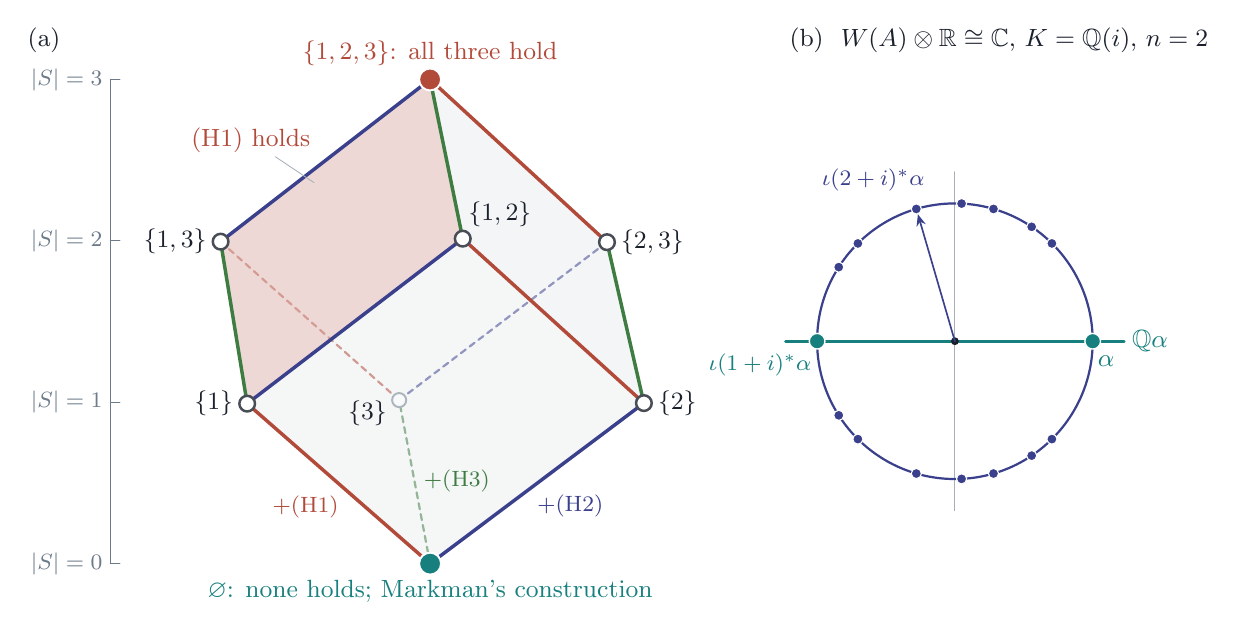
\begin{tikzpicture}[x=1cm,y=1cm,line join=round,line cap=round,
  font=\small,text=PInk]
  \path[fill=PSlate!14!white,fill opacity=0.26] (0.0000,-3.0885) -- (2.7152,-1.0496) -- (2.2465,0.9940) -- (-0.3928,-1.0116) -- cycle;
  \path[fill=PSlate!14!white,fill opacity=0.26] (0.0000,-3.0885) -- (-2.3230,-1.0566) -- (-2.6604,1.0005) -- (-0.3928,-1.0116) -- cycle;
  \path[fill=PSlate!14!white,fill opacity=0.26] (-0.3928,-1.0116) -- (-2.6604,1.0005) -- (0.0000,3.0603) -- (2.2465,0.9940) -- cycle;
  \draw[PGrass!70,line width=0.8pt,dash pattern=on 2.2pt off 1.8pt] (0.0000,-3.0885) -- (-0.3928,-1.0116);
  \draw[PClay!70,line width=0.8pt,dash pattern=on 2.2pt off 1.8pt] (-0.3928,-1.0116) -- (-2.6604,1.0005);
  \draw[PIndigo!70,line width=0.8pt,dash pattern=on 2.2pt off 1.8pt] (-0.3928,-1.0116) -- (2.2465,0.9940);
  \node[circle,fill=white,draw=PSlate!70,line width=0.7pt,inner sep=1.8pt] at (-0.3928,-1.0116) {};
  \path[fill=PClay!39!white,fill opacity=0.50] (-2.3230,-1.0566) -- (0.4146,1.0387) -- (0.0000,3.0603) -- (-2.6604,1.0005) -- cycle;
  \path[fill=PSlate!19!white,fill opacity=0.26] (2.7152,-1.0496) -- (0.4146,1.0387) -- (0.0000,3.0603) -- (2.2465,0.9940) -- cycle;
  \path[fill=PSlate!16!white,fill opacity=0.26] (0.0000,-3.0885) -- (-2.3230,-1.0566) -- (0.4146,1.0387) -- (2.7152,-1.0496) -- cycle;
  \draw[PClay,line width=1.25pt] (0.0000,-3.0885) -- (-2.3230,-1.0566);
  \draw[PIndigo,line width=1.25pt] (0.0000,-3.0885) -- (2.7152,-1.0496);
  \draw[PClay,line width=1.25pt] (2.7152,-1.0496) -- (0.4146,1.0387);
  \draw[PGrass,line width=1.25pt] (2.7152,-1.0496) -- (2.2465,0.9940);
  \draw[PClay,line width=1.25pt] (2.2465,0.9940) -- (0.0000,3.0603);
  \draw[PIndigo,line width=1.25pt] (-2.3230,-1.0566) -- (0.4146,1.0387);
  \draw[PGrass,line width=1.25pt] (-2.3230,-1.0566) -- (-2.6604,1.0005);
  \draw[PIndigo,line width=1.25pt] (-2.6604,1.0005) -- (0.0000,3.0603);
  \draw[PGrass,line width=1.25pt] (0.4146,1.0387) -- (0.0000,3.0603);
  \node[circle,fill=PTeal,draw=white,line width=0.7pt,inner sep=2.8pt] at (0.0000,-3.0885) {};
  \node[circle,fill=white,draw=PInk!80,line width=0.9pt,inner sep=2.0pt] at (2.7152,-1.0496) {};
  \node[circle,fill=white,draw=PInk!80,line width=0.9pt,inner sep=2.0pt] at (2.2465,0.9940) {};
  \node[circle,fill=white,draw=PInk!80,line width=0.9pt,inner sep=2.0pt] at (-2.3230,-1.0566) {};
  \node[circle,fill=white,draw=PInk!80,line width=0.9pt,inner sep=2.0pt] at (-2.6604,1.0005) {};
  \node[circle,fill=white,draw=PInk!80,line width=0.9pt,inner sep=2.0pt] at (0.4146,1.0387) {};
  \node[circle,fill=PClay,draw=white,line width=0.7pt,inner sep=2.8pt] at (0.0000,3.0603) {};
  \draw[PSlate,line width=0.45pt] (-4.060,-3.088) -- (-4.060,3.060);
  \draw[PSlate,line width=0.45pt] (-4.060,-3.088) -- (-3.940,-3.088);
  \draw[PSlate,line width=0.45pt] (-4.060,-1.039) -- (-3.940,-1.039);
  \draw[PSlate,line width=0.45pt] (-4.060,1.011) -- (-3.940,1.011);
  \draw[PSlate,line width=0.45pt] (-4.060,3.060) -- (-3.940,3.060);
  \draw[PSlate!60,line width=0.35pt] (6.665,-2.414) -- (6.665,1.886);
  \draw[PIndigo,line width=0.8pt] (6.665,-0.264) circle (1.750);
  \draw[PTeal,line width=1.0pt] (4.515,-0.264) -- (8.815,-0.264);
  \node[circle,fill=PIndigo,draw=white,line width=0.4pt,inner sep=1.3pt] at (8.415,-0.264) {};
  \node[circle,fill=PIndigo,draw=white,line width=0.4pt,inner sep=1.3pt] at (7.897,0.978) {};
  \node[circle,fill=PIndigo,draw=white,line width=0.4pt,inner sep=1.3pt] at (7.640,1.189) {};
  \node[circle,fill=PIndigo,draw=white,line width=0.4pt,inner sep=1.3pt] at (7.155,1.416) {};
  \node[circle,fill=PIndigo,draw=white,line width=0.4pt,inner sep=1.3pt] at (6.175,1.416) {};
  \node[circle,fill=PIndigo,draw=white,line width=0.4pt,inner sep=1.3pt] at (4.915,-0.264) {};
  \node[circle,fill=PIndigo,draw=white,line width=0.4pt,inner sep=1.3pt] at (6.175,-1.944) {};
  \node[circle,fill=PIndigo,draw=white,line width=0.4pt,inner sep=1.3pt] at (7.155,-1.944) {};
  \node[circle,fill=PIndigo,draw=white,line width=0.4pt,inner sep=1.3pt] at (7.640,-1.717) {};
  \node[circle,fill=PIndigo,draw=white,line width=0.4pt,inner sep=1.3pt] at (7.897,-1.507) {};
  \node[circle,fill=PIndigo,draw=white,line width=0.4pt,inner sep=1.3pt] at (6.750,1.484) {};
  \node[circle,fill=PIndigo,draw=white,line width=0.4pt,inner sep=1.3pt] at (5.433,0.978) {};
  \node[circle,fill=PIndigo,draw=white,line width=0.4pt,inner sep=1.3pt] at (5.433,-1.507) {};
  \node[circle,fill=PIndigo,draw=white,line width=0.4pt,inner sep=1.3pt] at (6.750,-2.012) {};
  \node[circle,fill=PIndigo,draw=white,line width=0.4pt,inner sep=1.3pt] at (5.190,0.677) {};
  \node[circle,fill=PIndigo,draw=white,line width=0.4pt,inner sep=1.3pt] at (5.190,-1.205) {};
  \node[circle,fill=PTeal,draw=white,line width=0.5pt,inner sep=2.0pt] at (8.415,-0.264) {};
  \node[circle,fill=PTeal,draw=white,line width=0.5pt,inner sep=2.0pt] at (4.915,-0.264) {};
  \node[circle,fill=PInk,inner sep=1.0pt] at (6.665,-0.264) {};
  \draw[PIndigo,line width=0.6pt,-{Stealth[length=4.2pt,width=3.4pt]}] (6.665,-0.264) -- (6.195,1.349);
  \draw[PSlate!60,line width=0.3pt] (-1.475,1.751) -- (-1.966,2.079);
  \node[text=PSlate,font=\footnotesize,inner sep=0pt] at (-4.616,-3.088) {$|S|=0$};
  \node[text=PSlate,font=\footnotesize,inner sep=0pt] at (-4.616,-1.039) {$|S|=1$};
  \node[text=PSlate,font=\footnotesize,inner sep=0pt] at (-4.616,1.011) {$|S|=2$};
  \node[text=PSlate,font=\footnotesize,inner sep=0pt] at (-4.616,3.060) {$|S|=3$};
  \node[text=PInk,font=\small,inner sep=0pt] at (7.224,3.560) {(b)\ \ $\HW(A)\otimes\RR\cong\CC$, $K=\QQ(i)$, $n=2$};
  \node[text=PInk,font=\small,inner sep=0pt] at (-4.903,3.560) {(a)};
  \node[text=PClay,font=\small,inner sep=0pt] at (0.000,3.398) {$\{1,2,3\}$: all three hold};
  \node[text=PTeal,font=\small,inner sep=0pt] at (-0.000,-3.439) {$\varnothing$: none holds; Markman's construction};
  \node[text=PInk,font=\small,inner sep=0pt] at (-2.747,-1.057) {$\{1\}$};
  \node[text=PInk,font=\small,inner sep=0pt] at (3.139,-1.050) {$\{2\}$};
  \node[text=PInk,font=\small,inner sep=0pt] at (-0.795,-1.178) {$\{3\}$};
  \node[text=PInk,font=\small,inner sep=0pt] at (0.887,1.354) {$\{1,2\}$};
  \node[text=PInk,font=\small,inner sep=0pt] at (-3.238,1.000) {$\{1,3\}$};
  \node[text=PInk,font=\small,inner sep=0pt] at (2.824,0.994) {$\{2,3\}$};
  \node[text=PClay,font=\footnotesize,inner sep=0pt] at (-1.581,-2.368) {$+$(H1)};
  \node[text=PIndigo,font=\footnotesize,inner sep=0pt] at (1.780,-2.361) {$+$(H2)};
  \node[text=PGrass,font=\footnotesize,inner sep=0pt] at (0.340,-2.036) {$+$(H3)};
  \node[text=PClay,font=\small,inner sep=0pt] at (-2.278,2.287) {(H1) holds};
  \node[text=PTeal,font=\small,inner sep=0pt] at (8.584,-0.517) {$\alpha$};
  \node[text=PTeal,font=\footnotesize,inner sep=0pt] at (4.191,-0.564) {$\iota(1+i)^{*}\alpha$};
  \node[text=PIndigo,font=\footnotesize,inner sep=0pt] at (5.628,1.781) {$\iota(2+i)^{*}\alpha$};
  \node[text=PTeal,font=\small,inner sep=0pt] at (9.142,-0.264) {$\QQ\alpha$};
\end{tikzpicture}
\end{document}
